\documentclass[../main.tex]{subfiles}

\pagestyle{main}
\renewcommand{\chaptermark}[1]{\markboth{\chaptername\ \thechapter}{}}

\begin{document}




\chapter{}
\section{Introduction to the Program (May / Rudenko)}
\begin{itemize}
    \item \marginnote{6/21:}Mainly given by Peter May.
    \item A far broader range of mathematics than any other REU.
    \item Things you have to do:
    \begin{enumerate}
        \item Soak up as much mathematics as you can.
        \item Work with a mentor to write a paper.
        \begin{itemize}
            \item You can work with people to write a joint paper?
            \item This is fairly unique to this REU.
        \end{itemize}
        \item Meet with your mentors at least twice a week.
    \end{enumerate}
    \item Don't be shy and unwilling to ask questions.
    \item Daniil Rudenko is in charge of the apprentice program.
    \item Apprentice program:
    \begin{itemize}
        \item An opportunity particularly early in one's mathematical career to explore mathematics.
        \item Asynchronous video lectures.
        \begin{itemize}
            \item Feel free to share with friends.
        \end{itemize}
        \item Problem solving.
        \begin{itemize}
            \item Problems that are not merely exercises but more difficult, interesting processes.
            \item Spend a couple hours a day thinking about these problems.
        \end{itemize}
    \end{itemize}
    \item Emphasis on relations between different subjects.
    \item They will be organizing social activities.
    \item Social meet and greet at 6:00 PM tonight.
    \item Breakout rooms:
    \begin{enumerate}
        \item Apprentice Program.
        \item Probability.
        \item Analysis and Dynamical Systems.
        \item Algebraic Topics.
        \item Main room: Algebraic Topology.
    \end{enumerate}
    \item More on the apprentice program:
    \begin{itemize}
        \item Daniil wants us to see much more than classical analysis/calculus. He doesn't see dividing lines between fields of mathematics.
        \item Bijections, binomial coefficients, Catalan numbers, etc. to start.
        \item Group of permutations, group of isometries of the plane, what a group is, etc.
        \item We can solve problems individually or in groups.
        \begin{itemize}
            \item Some problems will say not to collaborate.
        \end{itemize}
        \item Don't try to solve every problem. Don't try to solve everything fast; it's fine if you fail, if you just think about something for a couple hours that's interesting and don't get everywhere.
        \item On campus classes option for participants in Chicago.
        \item This week 10-11 AM Wed/Fri?
        \item Office hours 10-11 AM on Thursday.
        \item He will send an email with more information.
        \item Be consistent in whether you want to be on or off campus.
        \item You may attend whatever you want, but be careful: The apprentice program is your priority, so don't spend too much time on the other stuff.
        \begin{itemize}
            \item Follow Piazza groups to get links.
        \end{itemize}
        \item \LaTeX\ one solution each week.
    \end{itemize}
\end{itemize}



\section{Introduction to Complex Dynamics 1 (Calegari)}
\begin{itemize}
    \item Main focus: the Mandelbrot Set.
    \item Let $f_c:\C\to\C$ be the quadratic polynomial $f_c(z):=z^2+c$ where $c\in\C$ is a constant and $z\in\C$ is a variable.
    \begin{itemize}
        \item We study quadratics because they're the simplest nontrivial polynomial, i.e., one that displays the interesting phenomena of higher degree polynomials.
    \end{itemize}
    \item We want to understand the dynamics of $f_c$, i.e., what happens as we apply $f_c$ over and over again.
    \begin{itemize}
        \item In other words $z\to z^2+c\to (z^2+c)^2+c\to ((z^2+c)^2+c)^2+c\to\cdots$.
        \item Are there any special values of $z$ that have interesting characteristics?
    \end{itemize}
    \item \textbf{Fixed point}: A value $z$ such that $f_c(z)=z$.
    \begin{itemize}
        \item Fixed points of $f_c$ are equivalent to \textbf{roots} of $f_c-z$.
    \end{itemize}
    \item In this branch of mathematics, we don't care so much about factoring $f_c$ as much as we care about other special entities like fixed points and \textbf{critical points}.
    \item \textbf{Critical point}: A point where $\dv*{f_c}{z}=0$.
    \item We denote $z$ large by $|z|>>1$.
    \item Note that $z^2+c$ doesn't change the magnitude of $z$ that much unless $z$ is large.
    \begin{itemize}
        \item Essentially, if $|z|>>1$, then $|f_c(z)|>>|z|$.
    \end{itemize}
    \item Introduces composition notation: $z\to f_c(z)\to {f_c}^2(z)\to {f_c}^3(z)\to\cdots$\footnote{Sometimes, people also use a circled number in the superscript.}.
    \item If $z$ large, then the sequence $z,f_c(z),{f_c}^2(z),\dots$ converges to infinity.
    \item \textbf{Riemann Sphere}: The set $\hat{\C}:=\C\cup\infty$.
    \begin{itemize}
        \item Like an open set of complex numbers.
        \item In this case, we can think of infinity as a fixed point.
    \end{itemize}
    \item Any number whose absolute value is sufficiently big will converge to infinity.
    \item Introduces big $N$ convergence test.
    \item Infinity is an \textbf{attracting fixed point}, i.e. there exists an open neighborhood $U$ containing $\infty$ such that for all $z\in U$, ${f_c}^n(z)\to\infty$ as $n\to\infty$.
    \item \textbf{Filled Julia set}: The set $\{z:\text{the iterates }{f_c}^n(z)\text{ do not converge to }\infty\}$. \emph{Also known as} $\bm{K(f_c)}$.
    \begin{itemize}
        \item Equivalent to the set $\{z:\exists\text{ a constant }T\text{ s.t. }|{f_c}^n(z)|\leq T\ \forall\ n\}$.
    \end{itemize}
    \item The points that diverge to infinity are not that interesting; their divergence is their only property.
    \item Much more interesting are the points that do not diverge to infinity.
    \item Lemma: $K(f_c)$ is closed and bounded (i.e., compact).
    \begin{itemize}
        \item Proof: There exists $T$ (depending on $c$) such that if $|z|>T$, then $z\notin K(f_c)$. Furthermore, $z\in K(f_c)$ if and only if there exists $n$ such that $|{f_c}^n(z)|>T$. Let $U:=\{z:|z|>T\}$. This is open. Thus, $z\in K(f_c)\Longleftrightarrow z$ iterates ${f_c}^n(z)\in U$. Therefore, $K(f_c)=\C$, so $\bigcup_n{f_c}^n(U)$, i.e., $K(f_c)$ is closed.
        \item Bounded because numbers are not arbitrarily large. \emph{flesh out details?}
    \end{itemize}
    \item Calegari's proofs will be somewhat informal throughout the week; he hits the main points and leaves the details as an exercise to the student.
    \item Question: What other topological properties does the filled Julia set have?
    \begin{itemize}
        \item Is it possible that $K(f_c)=\emptyset$?
        \begin{itemize}
            \item No, it is not --- as a degree 2 polynomial, $f_c-z$ has at least one root, which will by necessity be a fixed point, i.e., not diverge to infinity, i.e., in the filled Julia set.
        \end{itemize}
        \item Could it be a finite set?
        \begin{itemize}
            \item No --- $K(f_c)$ is a \textbf{perfect set}.
            \item Uncountably infinite, too.
        \end{itemize}
        \item Is $K(f_c)$ connected?
        \begin{itemize}
            \item Sometimes.
        \end{itemize}
    \end{itemize}
    \item \textbf{Perfect set}: A set where every point in the set is a \textbf{nontrivial limit point} of the set.
    \begin{itemize}
        \item Example: A closed interval, \emph{others listed}.
    \end{itemize}
    \item \textbf{Nontrivial limit point}: A point $p$ in a set $A$ such that there is a nontrivial sequence (i.e., not a constant sequence, e.g., $p,p,p,\dots$) of points in $A$ that converge to $p$.
    \item \textbf{Not connected}: A set $X\subset\C$ such that there exist disjoint, open sets $U,V$ such that $X\subset U\cup V$, $X\cap U\neq\emptyset$, and $X\cap V\neq\emptyset$.
    \item \textbf{Mandlebrot set}: The set of complex numbers $c\in\C$ such that $K(f_c)$ is connected \emph{Also known as} $\bm{M}$.
    \item We can prove that $K(f_c)$ is connected if and only if the critical point of $f_c$ is an element of $K(f_c)$.
    \begin{itemize}
        \item Remember that critical points of $f_c$ are equivalent to zeroes of $f_c'$.
    \end{itemize}
    \item Note that critical points of $f_c:=z^2+c$ are equal to the roots of $f_c'=2z$, i.e., the elements of $\{0\}$.
    \item $K(f_c)$ is connected is equivalent to the sequence $0\to c\to c^2+c\to (c^2+c)^2+c\to\cdots$ is bounded (an absolute value).
    \begin{itemize}
        \item Thus, $c\in M$ is equivalent to the sequence $0\to c\to c^2+c\to (c^2+c)^2+c\to\cdots$ is bounded.
    \end{itemize}
    \item The Mandelbrot set is compact, too.
    \item Proposition: $K(f_c)$ is connected if and only if $0\in K(f_c)$.
    \begin{itemize}
        \item "Proof": $\C-K(f_c)=\bigcup_n{f_c}^{-n}(U)$ where $U$ is an open neighborhood of $\infty$, i.e., the set $\{z:|z|>T\}$.
        \item Let $X_n:=\C-{f_c}^{-n}(U)$, i.e., $X_0=\C-U$, so $K(f_c)=\bigcap_nX_n$.
        \item Cyclic map? $X_n$ getting "smaller" as $n$ increases? $X_{n+1}\subset X_n$.
        \item Assume $X_n=\text{little}$.
        \item Two cases: $X_n$ contains 0 and $X_n$ does not contain 0.
        \item Either every preimage of $X_n$ is connected or there is a $T$ such that for all $n\geq T$, $X_n$ is not connected.
    \end{itemize}
    \item Theorem (Douady-Hubbard): $M$ is connected.
\end{itemize}



\section{Harmonic Functions, Brownian Motion, and Analysis in the Plane 1 (Lawler)}
\begin{itemize}
    \item These topics will change week to week, so drop in at any point over the summer.
    \item Schedule:
    \begin{itemize}
        \item Lectures MWF at 2:30 PM.
        \item Group meeting Tuesday at 2:30 PM.
        \begin{itemize}
            \item Anybody can attend these!
        \end{itemize}
        \item No Zoom on Thursday, but there will be an opportunity to talk to Greg Lawler in person at the department of mathematics outside Eckhart when the weather is good.
    \end{itemize}
    \item Resources:
    \begin{itemize}
        \item Piazza --- look under the resources tab for lecture notes (with some exercises; these are very rough; gives you something to read with the lectures), other materials, etc.
        \item There is a 180 page book draft based on his REU lectures last summer.
        \begin{itemize}
            \item Do not share this.
        \end{itemize}
    \end{itemize}
    \item This math is at the border of analysis (basically advanced calculus) and probability.
    \begin{itemize}
        \item Lawler thinks of these as all basically the same subject.
    \end{itemize}
    \item We will work in $\R^2$.
    \item A lot of what Dr. Lawler does is often called Complex Analysis.
    \item Complex analysis allows you to get the results quicker even though they encapsulate ideas that are 100\% real; we're going to take a real-function perspective.
    \item Harmonic function notation:
    \begin{itemize}
        \item Domains $D$ are connected open sets that are subsets of $\R^2$.
        \item Mean value: $f:\R^2\to\R$ (continuous), or $f:D\to\R$.
        \item $z,w$ are points in $\R^2$, and we write $z=(x,y)$ where $x,y$ are the one-dimensional components.
        \item $B(z,\epsilon)=\{w:|z-w|<\epsilon\}$ is an open disk and $\partial\, B(Z,\epsilon)$ is the circle of radius $\epsilon$ about $z$.
    \end{itemize}
    \item If $B(z,\epsilon)\subset D$, then the (circular) mean value $MV(f;z,\epsilon)$ is the average rate of $f$ on $\partial B(z,\epsilon)$, i.e., the quantity
    \begin{equation*}
        \frac{1}{2\pi\epsilon}\int_{\{|w-z|=\epsilon\}}f(w)|\dd{w}|
    \end{equation*}
    where $|\dd{w}|$ is with respect to arc length.
    \item Let $(\cos\theta,\sin\theta)=\e[i\theta]$.
    \item \textbf{Harmonic function}: $f:D\to\R$ is harmonic if $f$ is continuous and for all $z\in D$ and every $\epsilon>0$ with $d(z,\partial D)>\epsilon$, then $f(z)=MV(f;z,\epsilon)$.
    \item Many applications, notably in physics wrt. heat.
    \begin{itemize}
        \item Consider $D$ describing a surface with heat. Fix the temperature at the boundary. Let $U(z)=\text{temperature at }z$ (in equilibrium).
        \item Then $U$ is harmonic on $D$.
    \end{itemize}
    \item We're going to understand the mean value in terms of the \textbf{Laplacian}.
    \item If $f:D\to\R$ is $C^2$ (the first and second derivatives exist and are continuous [either two derivatives in one variable or one derivative in both variables for $\R^2$]), then the Laplacian is defined by
    \begin{equation*}
        \Delta f(z) = f_{xx}(z)+f_{yy}(z)
    \end{equation*}
    \item Proposition: If $u$ is $C^2$ in $D$, then $\Delta u(z)=\lim_{\epsilon\to 0}4\cdot\frac{MV(u;z,\epsilon)-u(z)}{\epsilon^2}$.
    \item For ease, let's assume that $z=0=(0,0)$ and $u(z)=0$.
    \item Taylor polynomial (in several variables): If $z=(x,y)$, then
    \begin{equation*}
        u(z) = 0+u_x(0)x+u_y(0)y+\frac{1}{2}u_{xx}(0)x^2+\frac{1}{2}u_{yy}(0)y^2+u_{xy}(0)xy+\sigma(|z|^2)\footnotemark
    \end{equation*}
    \footnotetext{$\sigma$ is pronounced "little oh."}
    \begin{itemize}
        \item $u_x(0)MV(x;0,\epsilon)+u_y(0)MV(y;0,\epsilon)+u_{xy}(0)MV(xy;0,\epsilon)+\sigma(\epsilon^2)+\frac{1}{2}[u_{xx}(0)x^2+u_{yy}(0)y^2]$.
        \item Note that $u_{xx}(0)x^2=MV(x^2;0,\epsilon)$ and $u_{yy}(0)y^2=MV(y^2;0,\epsilon)$.
        \item You can use multivariable calculus, or you can observe that $MV(x^2;0,\epsilon)=MV(y^2;0,\epsilon)$, thus telling you that $MV(x^2;0,\epsilon)+MV(y^2;0,\epsilon)=MV(x^2+y^2;0,\epsilon)=\epsilon^2$.
        \item Since $|z|^2=\epsilon^2$, we have that $u(z)=\frac{1}{2}[\frac{1}{2}]$...
    \end{itemize}
    \item Proposition: A function $f:D\to\R$ is harmonic if and only if it is $C^2$ and $\Delta f(z)=0$ for all $z\in D$.
    \begin{itemize}
        \item Proof: Backwards direction first. We want to show that $C^2$ and $\Delta f(z)=0$ imply the mean value property. The mean value property clearly holds at $\epsilon=0$. Consider $MV(f;z,\epsilon)$ as a function of $\epsilon$. The derivative in $\epsilon$ ends up looking something like $\frac{1}{2\pi\epsilon}\int_\text{circle}\partial_nf(w)|\dd{w}|$ where $\partial_n$ is the normal direction.
        \item Using the divergence theorem, we have that the above is equal to $\int_\text{disk}\Delta f(w)\dd{w}$. Note that we sometimes write $\Delta f=\dd{w}(\nabla f)$ where $\nabla f=(f_x,f_y)$. Additionally, $\text{div}\,(\nabla f)=\partial_x(f_x)+\partial_y(f_y)$.
        \item Exercise: Show that if $u$ is harmonic, then $u$ is $C^2$.
    \end{itemize}
    \item The notion of probability comes in when we ask, "what is the `mean value' if we are not a disk viewed from the center?"
\end{itemize}



\section{The Mathematics of Playing Pool (Mazur)}
\begin{itemize}
    \item Main focus: Billiards in a polygon.
    \item The ball bounces off a side with the same angle of incidence it struck it with. If the ball hits the corner, it stops (maybe it fell into a pocket).
    \item \textbf{Billiards}: Start with a polygon in the plane. Shoot a billiard ball, thought of as a point mass, ...
    \item Rectangular tables are fully understood, but other polygons are harder. Curved sides are even more complicated.
    \item Connection to physics: Ehrenfest windtree model (by Paul and Tatjana Ehrenfest, 1912).
    \item One thing people study is the diffusion rate of a random particle. This means that if you take a random particle and follow it for a long time $t$, how far is it from where it started? What people know is that a typical particle is about distance $t^{2/3}$ away.
    \item Another example: Take two point masses with positions $0\leq x_1\leq x_2\leq 1$ on the unit interval $[0,1]$. Suppose their masses are $m_1,m_2$ and they move with velocities $v_1,v_2$, respectively. They collide with each other and with the barriers at 0 and 1. Momentum and energy are conserved.
    \begin{itemize}
        \item We can convert this to billiards in a right triangle with the observations that energy and speed are related and momentum and angle of incidence are related.
    \end{itemize}
    \item Billiards are important examples of \textbf{dynamical systems} where one studies behavior of objects under a deterministic system (initial position and velocity define motion for the rest of time).
    \item Billiards questions:
    \begin{itemize}
        \item Are there periodic orbits?
        \item How does a typical orbit behave in the long term? Is it dense? Is it equidistributed?
        \item Illumination problem (can you get from any point to any other?).
    \end{itemize}
    \item Periodic orbits:
    \begin{itemize}
        \item There are periodic orbits in acute triangles.
        \item Drop perpendiculars; use Euclidean geometry to prove.
        \item It is unknown if a general obtuse triangle has a periodic orbit. This is considered to be one of the big unsolved problems in dynamics\footnote{Can we consider the set of all possible initial positions and directions and see what converges to what?}.
    \end{itemize}
    \item Equidistribution and Ergodicity:
    \begin{itemize}
        \item ...
    \end{itemize}
    \item Rational billiards is much more well-defined. Every rational table has periodic orbits.
    \item Most paths equidistribute.
    \item Illumination problem:
    \begin{itemize}
        \item Now imagine you put a light source at a point on your table. The walls are mirrors and a light beam bounces of the mirror with angle of incidence equal to angle of reflection. Is every point illuminated? In other words, can you get from any point to any other? Not in a Penrose unilluminable room (a region is dark in this elliptical room).
        \item Polygon example from Tokarski in the 1980s (a zero-dimensional point is unilluminable).
        \item Within the last 5 years: For any rational billiard, there are at most a finite number of unilluminable points.
    \end{itemize}
    \item Unfolding billiards boards.
    \item If the slope of the line on a torus is rational, it closes up. If the slope of the line on a torus is irrational, it does not close but is equidistributed.
    \item For a square, when we glue the unfolded version together, we get a genus 1 surface (a torus).
    \item For a triangle with angles $\frac{\pi}{2}$, $\frac{\pi}{8}$, and $\frac{3\pi}{8}$, the unfolded version can be glued together into a genus 2 surface.
    \item Ergodicity:
    \begin{itemize}
        \item A common notion in mathematics is that of irreducibility.
        \item In our context, irreducible (or ergodic) means you cannot divide your table $X$ nontrivially into 2 pieces $X=X_1\cup X_2$ so that if you start with a point in $X_1$ and you move in a straight line, you stay in $X_1$ and if you start in $X_2$ you stay there.
        \item In other words, there are no invariant sets.
    \end{itemize}
    \item Proves the Kronecker-Weyl theorem.
\end{itemize}



\section{Lecture 1.1: Bijections and Permutations}
\begin{itemize}
    \item Consider the statement $4=4$.
    \begin{itemize}
        \item "Four is an abstraction for any set of four elements."
        \item Thus, $4=4$ implies that $\{\text{lion},\text{cat},\text{tiger},\text{cheetah}\}=\{\text{burger},\text{pizza},\text{pasta},\text{borsh}\}$, for instance, but in what sense are these sets similar? They are related because there exists a bijection between them. Note, however, that there are $4!=24$ possible bijections between these two sets.
    \end{itemize}
    \item Let $A,B$ be sets and $f:A\to B$ be a function (or map).
    \begin{figure}[h!]
        \centering
        \begin{tikzpicture}
            \small
            \draw (-1,0) ellipse (5mm and 9mm) node[above=9mm]{$A$};
            \draw (1,0)  ellipse (5mm and 9mm) node[above=9mm]{$B$};

            \footnotesize
            \fill (-1,0.6)  circle (1.5pt);
            \fill (-1,0.2)  circle (1.5pt);
            \fill (-1,-0.2) circle (1.5pt);
            \fill (-1,-0.6) circle (1.5pt);
            \fill (1,0.6)   circle (1.5pt);
            \fill (1,0.2)   circle (1.5pt);
            \fill (1,-0.2)  circle (1.5pt);
            \fill [rex] (1,-0.6)  circle (1.5pt);

            \draw [semithick,-stealth,shorten >=2pt] (-1,0.6) -- node[above=2mm]{$f$} (1,0.2);
            \draw [semithick,-stealth,shorten >=2pt] (-1,0.2) -- (1,0.6);
            \draw [semithick,rey,-stealth,shorten >=2pt] (-1,-0.2) -- (1,-0.2);
            \draw [semithick,rey,-stealth,shorten >=2pt] (-1,-0.6) -- (1,-0.2);
        \end{tikzpicture}
        \caption{A function that is neither injective nor surjective.}
        \label{fig:notInjectSurject}
    \end{figure}
    \begin{itemize}
        \item $f$ is \textbf{injective} if for all $a_1,a_2\in A$, $f(a_1)=f(a_2) \Longrightarrow a_1=a_2$.
        \item $f$ is \textbf{surjective} if for every element $b\in B$, there exists an $a\in A$ such that $f(a)=b$.
        \item $f$ is \textbf{bijective} if it is surjective and injective.
        \begin{itemize}
            \item These are one-to-one correspondances.
        \end{itemize}
        \item The function $f$ in Figure \ref{fig:notInjectSurject} is a function because it maps every element of $A$ to an element of $B$. However, it is not injective because the mappings indicated in \textcolor{rey}{light red} map two distinct elements of $A$ to the same element of $B$. Likewise, it is not surjective because the element of $B$ drawn in \textcolor{rex}{dark red} is not the image of any element of $A$ under $f$. Because $f$ is neither injective nor surjective, it is not bijective.
    \end{itemize}
    \item If there exists a bijection between the set $A$ and the nice set $[n]=\{1,2,\dots,n\}$, we say that $|A|=n$.
    \item Example:
    \begin{itemize}
        \item Consider the sets $A=\N$ and $B=\{2k\mid k\in\N\}$.
        \item Define $f:A\to B$ by $f(x)=2x$. $f$ is a bijection.
        \item Thus, $|A|=|B|$ despite the intuitive sense that $|B|$ should be half $|A|$.
    \end{itemize}
    \item Sets in bijection with $\N$ are called \textbf{countable}, and we write $|A|=\aleph_0$.
    \begin{itemize}
        \item We can show that $|\Q|=\aleph_0$ and $|\R|\neq\aleph_0$.
    \end{itemize}
    \item \textbf{Permutation}: A bijection $\sigma:S\to S$, where $S=\{1,\dots,n\}$.
    \item Examples:
    \begin{itemize}
        \item $n=1$:
        \begin{itemize}
            \item There exists a unique permutation of the set, which is an identity.
        \end{itemize}
        \item $n=2$:
        \begin{itemize}
            \item There are two different bijections here.
            \item They are denoted by the following matrices.
            \begin{align*}
                \sigma &=
                \begin{pmatrix}
                    1 & 2\\
                    1 & 2\\
                \end{pmatrix}&
                \sigma &=
                \begin{pmatrix}
                    1 & 2\\
                    2 & 1\\
                \end{pmatrix}
            \end{align*}
        \end{itemize}
        \item $n=3$:
        \begin{itemize}
            \item Listing\footnote{Dr. Rudenko also shows function diagrams and directed graphs (see Figure \ref{fig:directedGraphS8}).} the elements of $\Ss_3$:
            \begin{align*}
                \Ss_3 &= \left\{
                    \begin{pmatrix}
                        1 & 2 & 3\\
                        1 & 2 & 3\\
                    \end{pmatrix},
                    \begin{pmatrix}
                        1 & 2 & 3\\
                        2 & 1 & 3\\
                    \end{pmatrix},
                    \begin{pmatrix}
                        1 & 2 & 3\\
                        3 & 2 & 1\\
                    \end{pmatrix},
                    \begin{pmatrix}
                        1 & 2 & 3\\
                        1 & 3 & 2\\
                    \end{pmatrix},
                    \begin{pmatrix}
                        1 & 2 & 3\\
                        2 & 3 & 1\\
                    \end{pmatrix},
                    \begin{pmatrix}
                        1 & 2 & 3\\
                        3 & 1 & 2\\
                    \end{pmatrix}
                \right\}\\
                &= \left\{
                    \permtwo{1}{2}{3},
                    \permtwo{2}{1}{3},
                    \permtwo{3}{2}{1},
                    \permtwo{1}{3}{2},
                    \permtwo{2}{3}{1},
                    \permtwo{3}{1}{2}
                \right\}
                % &= \left\{
                %     \tikz[baseline={(0,0.4)}]{
                %         \node (1) at (0,0.8) {1} edge [out=150,in=120,loop] ();
                %         \node (2) at (0.8,0.8) {2} edge [out=30,in=60,loop] ();
                %         \node (3) at (0,0) {3} edge [out=-150,in=-120,loop] ();
                %     }
                % \right\}
            \end{align*}
            \item There are different important classes of permutations --- the first one listed is an identity, the next three listed are identities for one object and \textbf{cycles} of length two for the other two, and the last two are \textbf{cycles} of length three.
            \item $|\Ss_3|=6$.
        \end{itemize}
    \end{itemize}
    \item More generally, the numbers in the first row are the numbers 1 through $n$ and the numbers in the second row are those to which the bijection maps each number:
    \begin{equation*}
        \sigma =
        \begin{pmatrix}
            1 & 2 & \cdots & n\\
            \sigma(1) & \sigma(2) & \cdots & \sigma(n)\\
        \end{pmatrix}
    \end{equation*}
    \item We denote by $\Ss_n$ the set of permutations of $S=\{1,\dots,n\}$.
    \item Exercises:
    \begin{enumerate}
        \item Draw all permutations in $\Ss_4$.
        \item Prove that $|\Ss_n|=n!$.
        \begin{itemize}
            \item Perhaps by induction? Trivial for the base case of 0. Then if true for $n$, we can map $n+1$ to $n+1$ possible numbers, so we divide into $n+1$ cases. If $\sigma(n+1)=1$, then we know by the inductive hypothesis that we can permute the remaining $n$ numbers in $n!$ ways. Thus, the number of permutations is $\underbrace{n!+n!+\cdots+n!}_{n+1\text{ times}}=(n+1)\cdot n!=(n+1)!$.
        \end{itemize}
    \end{enumerate}
    \item Note that in $\S_3$, permutations $\sigma(2,1,3)$, $\sigma(3,2,1)$, and $\sigma(1,3,2)$ are considered odd and the others are considered even.
    \begin{itemize}
        \item This classification is based on the number of crossings in the function diagrams.
    \end{itemize}
\end{itemize}



\section{Lecture 1.2: The Group of Permutations}
\begin{itemize}
    \item \textbf{Composition}: The function $g\circ f:A\to C$ defined by the map $(g\circ f)(a)=g(f(a))$, where $A,B,C$ are sets and $f:A\to B$ and $g:B\to C$ are functions.
    \item The composition of two bijections is a bijection (Proposition 1.26).
    \item We can compose permutations to get new (or the same) permutations.
    \begin{itemize}
        \item Example: If $\sigma=(2,1,3)$ and $\tau=(1,3,2)$, then $\tau\cdot\sigma=(3,1,2)$.
    \end{itemize}
    \item This new function is known as a \textbf{product of permutations}.
    \item If you do this many times to the same permutation, you construct the power of a permutation.
    \item Example:
    \begin{itemize}
        \item Consider $\sigma(3,5,1,2,4)$.
        \item If we draw this out, then we can see that there is a cycle of length two and a cycle of length 3.
        \item Thus, $\sigma^{100}=(1,5,3,2,4)$. $100\%2=0$, so $\sigma^{100}=i$ with respect to the $3,1$ cycle. Additionally, $100\%3=1$, so $\sigma^{100}=\sigma$ with respect to the $5,2,4$ cycle.
        \item Also note that $\sigma^{2\cdot 3}=\sigma^6=i$, where $i$ is the identity permutation.
    \end{itemize}
    \item Multiplication of permutations is associative.
    \item Thus, we can construct multiplication tables.
    \item Example:
    \begin{table}[h!]
        \centering
        \renewcommand{\arraystretch}{1.2}
        \begin{tabular}{c|cc}
                     & $\bm{e}$ & $\bm{x}$\\
            \hline
            $\bm{e}$ & $e$      & $x$\\
            $\bm{x}$ & $x$      & $e$\\
        \end{tabular}
        \caption{Multiplication table for $\Ss_2$.}
        \label{tab:S2MultiplicationTable}
    \end{table}
    \begin{itemize}
        \item This holds where $e=(1,2)$ and $x=(2,1)$.
    \end{itemize}
    \item \textbf{Identity}: The function $\text{id}_A:A\to A$ defined by $\text{id}_A(a)=a$, where $A$ is a set.
    \begin{itemize}
        \item $\text{id}_{[n]}=(1,2,\dots,n)=e\in\Ss_n$.
        \begin{itemize}
            \item $e$ is also known as the \textbf{trivial permutation} or \textbf{identity permutation}.
        \end{itemize}
        \item For all $\sigma\in\Ss_n$, $\sigma\cdot e=e\cdot\sigma=\sigma$.
    \end{itemize}
    \item \textbf{Inverse}: The function $f^{-1}:B\to A$ corresponding to the function $f:A\to B$ having the properties that $f\circ f^{-1}=\text{id}_B$ and $f^{-1}\circ f=\text{id}_A$.
    \item $f^{-1}$ exists iff $f$ is a bijection (Proposition 1.27).
    \item Note that it's often easier to check the two inverse properties than to confirm that $f$ is bijective.
    \item Since permutations are bijections, all permutations have inverses.
    \begin{itemize}
        \item If $\left(
            \begin{smallmatrix}
                1 & 2 & 3 & 4 & 5\\
                3 & 4 & 1 & 2 & 5\\
            \end{smallmatrix}
            \right)=\sigma\in\Ss_5
        $, then $
            \sigma^{-1}=\left(
            \begin{smallmatrix}
                3 & 4 & 1 & 2 & 5\\
                1 & 2 & 3 & 4 & 5\\
            \end{smallmatrix}
            \right)=\left(
            \begin{smallmatrix}
                1 & 2 & 3 & 4 & 5\\
                3 & 4 & 1 & 2 & 5
            \end{smallmatrix}
            \right)
        $.
        \item Note that in this case $\sigma=\sigma^{-1}$, indicating the existence of only 1- and 2-cycles.
    \end{itemize}
    \item \textbf{Group}: A set $G$ along with a map $G\times G\to G$.
    \item If the following properties hold, then a collection of objects is a group.
    \begin{enumerate}
        \item Associativity: For all $g_1,g_2,g_3\in G$, $(g_1g_2)g_3=g_1(g_2g_3)$.
        \item Identity: There exists a special element $e\in G$ such that for any $g\in G$, $g\circ e=e\circ g=g$.
        \item Inverse: For all $g\in G$, there exists $g^{-1}\in G$ such that $g\circ g^{-1}=g^{-1}\circ g=e$.
    \end{enumerate}
    \item Examples:
    \begin{itemize}
        \item $\Ss_n$ is a group.
        \item $\Z$ and addition is a group.
        \item $\Q$ and multiplication is a group (notably, $\Z$ and multiplication is not).
    \end{itemize}
\end{itemize}



\section{Introduction to Complex Dynamics 2 (Calegari)}
\begin{itemize}
    \item \marginnote{6/22:}Picking up from yesterday on the proof of the proposition, $K(f_c)$ is connected iff $0\in K(f_c)$.
    \begin{itemize}
        \item Recall that 0 is the unique critical point.
        \item Also recall that $U$ is the set that contains only elements with sufficiently big absolute values, big enough so that $f_c(U)\subset U$.
        \item Define $X_0=\C-U$, $X_{n+1}={f_c}^{-n}(X_n)$.
        \begin{itemize}
            \item Each $X_n$ is compact, and $K(f_c)$ is equal to the intersection of all $X_n$, therefore compact in and of itself.
        \end{itemize}
        \item Thus, $K(f_c)$ is connected iff every $X_n$ is connected.
        \item Key point: If $0\in K(f_c)$, then each $X_n$ is a disk; otherwise, some $X_n$ is not a disk.
        \item Fact: Every point in $\C$ has exactly 2 preimages under $f_c$ except for the critical value $c=f_c(0)$ since $f_c$ is a degree 2 polynomial.
        \item Assume $X_n$ is a disk. If $X_n$ contains the critical value, then $X_{n+1}$ is a disk; otherwise, not (in fact, it will be disconnected).
    \end{itemize}
    \item Under $f_c$, the preimage of a circle not containing the critical value is either 2 circles, each of which maps one-to-one, or a single circle mapping two-to-one.
    \begin{itemize}
        \item Suppose that the preimage of the boundary of the circles is two distinct circles.
        \item By continuity, concentric circles narrowing down within the original set narrow down within the other two circles.
        \item Each point in $X_n$ has exactly two preimages iff $c\notin X_n$.
        \item As we make smaller and smaller circles, than we can split our one-circle preimage into two disconnected subsets.
    \end{itemize}
    \item Today: The theory of Julia sets for holomorphic functions in general.
    \item Let $f$ be a \textbf{holomorphic} map from $\hat{\C}$ to itself.
    \item Every such $f$ has finitely many 0s and poles ($\infty$s).
    \item Therefore, $f$ is a rational function, i.e., a ratio of polynomials. Symbolically, $f(z)=\frac{p(z)}{q(z)}$ for some polynomials $p,q$.
    \item To talk about Julia sets, we need some definitions.
    \item \textbf{Normal family}: Let $U$ be an open subset of the Riemann sphere $\hat{\C}$, and let $F$ be a family of holomorphic functions $f:U\to\hat{\C}$. $F$ is \textbf{normal} if its closure (in the space of all holomorphic functions from $U$ to $\hat{C}$) is compact.
    \begin{itemize}
        \item In other words, if ever infinite sequence $f_n\in F$ has a subsequence that converges locally uniformly to some limit $g:U\to\hat{\C}$.
    \end{itemize}
    \item Normality is local.
    \item Proposition: Suppose $F$ is a family of holomorphic functions defined on $U$, and suppose for all $p\in U$, there exists open $p\in V\subset U$ such that $F|_V$ is normal. Then $F|_U$ is normal.
    \begin{itemize}
        \item Proof 1: Diagonal argument.
        \item Proof 2: ???
    \end{itemize}
    \item \textbf{Julia set}: Let $f$ be a holomorphic map from $\hat{\C}$ to itself. Let $\mathcal{F}:=\{f^n\mid n\in\N\}$. The Fatou set $\Omega_f:\subset\hat{\C}$ is the open subset whose $\mathcal{F}$ is normal. It is equal to the union of all $U$ where $F|_U$ is normal. Thus, $\Omega_f$ is open and $\mathcal{F}|_{\Omega_f}$ is normal. The \textbf{Julia set} $J_f:\subset\hat{\C}$ is $\hat{C}-\Omega_f$, i.e., $p\in J_f$ iff for all $U$ containing $p$, $F|_U$ is not normal on $U$.
    \begin{itemize}
        \item Hence, $J_f$ is compact.
    \end{itemize}
    \item Example: Let's let $p$ be a fixed point for $f$.
    \begin{itemize}
        \item $p$ is an attracting fixed point if $|f'(p)|<1$. $p$ is super attracting if $|f'(p)|=0$.
        \item Example:
        \begin{itemize}
            \item If $f$ is a polynomial of degree at least 2, then $\infty$ is a super attracting fixed point.
        \end{itemize}
        \item If we take a sufficiently small neighborhood of $p$, then $f$ shrinks and rotates the neighborhood a little bit.
        \item \textbf{Basin of attraction} of $p$.
        \item \textbf{Immediate basin of attraction} of $p$ is the connected component of the basin of attraction of $p$.
    \end{itemize}
    \item If $f$ is a polynomial, then $K(f_c)$ is equal to the complement of the basin of infinity.
    \item "Most" "typical" $f$ have $\Omega_f=\bigcup\text{basins of attraction of attracting periodic orbits}$.
    \begin{itemize}
        \item Furthermore: every immediate basin of an attracting periodic orbit contains at least one critical point.
        \item A rational map of degree $d$ (the maximum of the degrees of polynomials $p,q$) has $2d-2$ critical points.
    \end{itemize}
    \item Theorem: The closure of the set of repelling periodic orbits (i.e., $p$ with $f^n(p)=p$ and $|(f^n)'(p)|>1$) is $J_f$.
\end{itemize}



\section{Coambiguous Concepts 1 (May)}
\begin{itemize}
    \item Categories can inscribe things of different types.
    \item Categories can be interesting mathematical objects in and of themselves much like rings, groups, etc.
    \item Whenever you define an object, you should define a notion of a morphism (or map) between objects.
    \item Morphisms have compositions and identities.
    \item A monoid is a category with one object. A category is a monoid with many objects!
    \item Today: Category theory.
    \item \textbf{Poset}: A \underline{p}artially \underline{o}rdered \underline{set}, i.e., one that is transitive, reflexive, and antisymmetric ($A\leq B\text{ and }A\geq B\Longleftrightarrow A=B$).
    \item \textbf{Small category}: A category that has a set of objects as opposed to a class of objects. \emph{Also known as} \textbf{kitty category}, \textbf{kittygory}.
\end{itemize}



\section{Lecture 1.3: Cyclic Structure of a Permutation}
\begin{itemize}
    \item Let $
        \sigma=\left(
            \begin{smallmatrix}
                1 & 2 & 3 & 4 & 5 & 6 & 7 & 8\\
                7 & 3 & 4 & 2 & 6 & 5 & 1 & 8\\
            \end{smallmatrix}
        \right)\in\Ss_8
    $.
    \item Consider the directed graph representation.
    \begin{figure}[h!]
        \centering
        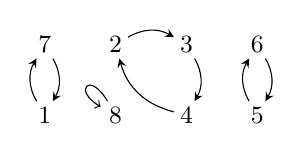
\begin{tikzpicture}[scale=0.9,inner sep=2pt]
            \small
            \node (1) at (0,0) {1};
            \node (7) at (0,1) {7}
                edge [stealth-,bend right=30] (1)
                edge [-stealth,bend left=30] (1)
            ;
            \node (2) at (1,1) {2};
            \node (3) at (2,1) {3}
                edge [stealth-,bend right=30] (2)
            ;
            \node (4) at (2,0) {4}
                edge [stealth-,bend right=30] (3)
                edge [-stealth,bend left=30] (2)
            ;
            \node (8) at (1,0) {8}
                edge [out=120,in=150,loop] ()
            ;
            \node (5) at (3,0) {5};
            \node (6) at (3,1) {6}
                edge [stealth-,bend right=30] (5)
                edge [-stealth,bend left=30] (5)
            ;
        \end{tikzpicture}
        \caption{Directed graph of a permutation in $\Ss_8$.}
        \label{fig:directedGraphS8}
    \end{figure}
    \begin{itemize}
        \item Note that this is a graph because it has points connected by edges, it is directed because the edges have a direction (they are arrows/mappings), and it has some loops and some multiple edges (points with more than one edge).
        \item There are four cycles in this graph (a 1-cycle, two 2-cycles, and a 3-cycle).
    \end{itemize}
    \item \textbf{Cycle}: A permutation $\sigma=(i_1,\dots,i_k)\in\Ss_n$, where $1\leq i_1\leq\cdots\leq i_k\leq n$, such that $\sigma(i_j)=i_{j+1}$, $\sigma(i_k)=i_1$, and $\sigma(s)=s$ for all $s\in[n]\setminus\{i_1,\dots,i_k\}$.
    \item For example, $\sigma=(1,3,5)\in\Ss_5$ is the permutation $
        \sigma=\left(
            \begin{smallmatrix}
                1 & 2 & 3 & 4 & 5\\
                3 & 2 & 5 & 4 & 1\\
            \end{smallmatrix}
        \right)
    $.
    \item \textbf{Length} (of a cycle): The value $k$ in the above definition.
    \item \textbf{Support} (of a cycle): The set of indices $\{i_1,\dots,i_k\}$ in the above definition.
    \item \textbf{Transposition}: A cycle $(i,j)\in\S_n$, where $i,j\in[n]$ are distinct.
    \item Thus, $\Ss_3=\{e,(1,2),(2,3),(1,3),(1,2,3),(1,3,2)\}$.
    \item Exercise:
    \begin{itemize}
        \item Count the number of transpositions in $\Ss_n$.
        \item Prove that every permutation is a product of transpositions.
        \begin{itemize}
            \item Consider crossings in the function diagram! Relate to braids from knot theory.
            \item For instance, $
                \left(
                    \begin{smallmatrix}
                        1 & 2 & 3 & 4 & 5\\
                        3 & 4 & 1 & 2 & 5\\
                    \end{smallmatrix}
                \right)=(1,4)(2,4)(1,3)(2,3)
            $.
        \end{itemize}
    \end{itemize}
    \item \textbf{Independent} (cycles): Two cycles $\sigma_1,\sigma_2\in\Ss_n$ with disjoint supports.
    \item \textbf{Dependent} (cycles): Two cycles that are not independent.
    \item Propositions:
    \begin{enumerate}
        \item Every permutation is a product of independent cycles.
        \begin{itemize}
            \item In the directed graph corresponding to $\sigma$, every vertex has on incoming edge.
            \item There exists a smallest $k$ such that $\sigma^k(i)=i$.
            \item \emph{Return to this?}
        \end{itemize}
        \item Independent cycles commute with each other.
        \begin{itemize}
            \item Obvious: Consider $c_1,c_2$ independent. Then
            \begin{equation*}
                c_1c_2(i) =
                \begin{cases}
                    c_1(i) & i\text{ is in the support of }c_1\\
                    c_2(i) & i\text{ is in the support of }c_2\\
                    i      & i\text{ is in the support of neither}
                \end{cases}
            \end{equation*}
        \end{itemize}
    \end{enumerate}
\end{itemize}



\section{Lecture 1.4: Binomial Coefficients}
\begin{itemize}
    \item Start with the set $S=\{1,\dots,n\}$. Denote by $2^S$ the set of subsets of $S$.
    \begin{itemize}
        \item If $n=2$, then $2^S=\{\emptyset,\{1,2\},\{1\},\{2\}\}$ has four elements.
    \end{itemize}
    \item Proposition: $|2^S|=2^{|S|}$.
    \begin{itemize}
        \item Consider the set $S=\{1,2,3,4,5,6\}$.
        \item Identify subsets of $S$ with a code, exemplified by $\{1,3,5\}\mapsto(1,0,1,0,1,0)$.
        \item Based on this, construct a map $f$ which sends $2^S\to$ the set of sequences of $0,1$ of length $n$. In other terms, map each subset $A\in 2^S$ to a sequence $(s_1,\dots,s_n)$ where
        \begin{equation*}
            s_i =
            \begin{cases}
                0 & i\notin A\\
                1 & i\in A
            \end{cases}
        \end{equation*}
        \item For example, $f(\emptyset)=(0,0,0,0,0,0)$ and $f(S)=(1,1,1,1,1,1)$.
        \item Note that $f$ is a bijection.
        \item Since the set of all sequences of $0,1$ of length $n$ (more commonly denoted by $\{0,1\}^n$) clearly has $2^n$ elements and $2^S$ is in bijective correspondence with this set, we know that $2^S$ has $2^{|S|}=2^n$ elements.
    \end{itemize}
    \item Note that coding subsets by sequences is very important in computer science and mathematics.
    \item Geometric model: Vertices of a line segment give you subsets of a set with 1 element, vertices of a square give you subsets of a set with 2 elements, vertices of a cube give you subsets of a set with 3 elements, \dots
    \item If $A\in 2^S$ and $f(A)=(a_1,\dots,a_n)$, then $|A|=\sum_{i=1}^na_i$.
    \item If $0\leq k\leq n$, then $\binom{n}{k}$ is the number of subsets of size $k$ in a set of size $n$.
    \item Proposition: $\binom{n}{k}=\frac{n!}{k!(n-k)!}$.
    \begin{itemize}
        \item $\binom{n}{k}\cdot k!$ is the number of subsets of size $k$ and the orderings of their elements.
        \item But this is the same as choosing the first element from among $n$ elements, the second from among the remaining $n-1$ elements and so on until $n-k+1$, i.e.,
        \begin{align*}
            \binom{n}{k}\cdot k! &= n\cdot(n-1)\cdots(n-k+1)\\
            &= \frac{n!}{(n-k)!}
        \end{align*}
    \end{itemize}
    \item By convention, $\binom{n}{0}=1=\binom{n}{n}$.
    \item Proposition: $\binom{n}{k}=\binom{n}{n-k}$.
    \begin{itemize}
        \item Follows from the previous proposition.
        \item Alternatively, we can seek to show that the number of subsets of size $k$ is equal to the number of subsets of size $n-k$. But since these are inverse maps, they obviously are.
    \end{itemize}
    \item Proposition: $\binom{n}{k}=\binom{n-1}{k-1}+\binom{n-1}{k}$.
    \begin{itemize}
        \item Follows from the factorial formula.
        \item Conceptually:
        \begin{itemize}
            \item Divide the set of subsets of $S$ of size $k$ into those that contain $n$ and those that do not contain $n$.
            \item The subsets of size $k$ that do not contain $n$ is equal to the subsets of $S\setminus\{n\}$ of size $k$, i.e., $\binom{n-1}{k}$.
            \item The subsets of size $k$ the do contain $n$ are in bijection with the subsets of size $k-1$ in $S\setminus\{n\}$, i.e., $\binom{n-1}{k-1}$.
        \end{itemize}
    \end{itemize}
    \item Introduces Pascal's triangle.
    \begin{itemize}
        \item The symmetry of Pascal's triangle follows from the formula $\binom{n}{k}=\binom{n}{n-k}$.
    \end{itemize}
    \item Theorem (Binomial Formula):
    \begin{align*}
        (a+b)^n &= \binom{n}{0}a^n+\binom{n}{1}a^{n-1}b+\cdots+\binom{n}{n}b^n\\
        &= \sum_{k=0}^n\binom{n}{k}a^{n-k}b^k
    \end{align*}
    \begin{itemize}
        \item Induction proof: Left as an exercise.
        \item $(a+b)^n=\underbrace{(a+b)(a+b)\cdots(a+b)}_{n\text{ times}}=$ a sum of monomials, e.g., $aabbaba$. We get each monomial by choosing $a$ or $b$ from each parentheses. Thus, $(a+b)^n=\sum_{A\subset\{1,\dots,n\}=S}a^{|A|}b^{|S\setminus A|}$.
    \end{itemize}
    \item Corollary: If $a=b=1$, then $2^n=(1+1)^n=\sum_{k=0}^n\binom{n}{k}1^{n-k}1^k=\sum_{k=0}^n\binom{n}{k}$.
\end{itemize}



\section{Problem Session 1}
\begin{itemize}
    \item \marginnote{6/23:}The goal is to get you to think about math all the time. You should let problems sit in your head for a week; no expectation of solving them, but just thinking about it.
    \item Typo in 5a. Nobody knows what problem 4 means.
    \item If you're ever lost on a permutation problem, just draw out the connected graph.
    \item Prove any permutation is a product of adjacencies.
    \item 5d technically proves 5c, but there is a nicer formula for 5c that he would rather we find.
\end{itemize}




\end{document}